\section{Agent Framework Evolution: From ReAct to the Model-Native OS}
\label{sec:agentevolution}

An \textit{agent framework} is a software system built around a large language model that enables autonomous planning, tool invocation, state management, and the completion of complex multi-step tasks.
Between 2022 and 2025, these frameworks have undergone a systematic evolution that closely mirrors the historical progression of operating systems: from single-task batch processing, through multiprogramming and time-sharing, to protected and governed execution environments.
This section traces five distinct generations of this evolution, examining each along three dimensions: its \textbf{core architectural contribution}, its \textbf{representative systems and their concrete mechanisms}, and its \textbf{structural correspondence to classical operating-system history}.

Figure~\ref{fig_agent_timeline} presents a timeline of the five-generation evolution.
\begin{figure}[htbp]
\centering
%% ── Gemini-generated image version (active) ──────────────────────────────────
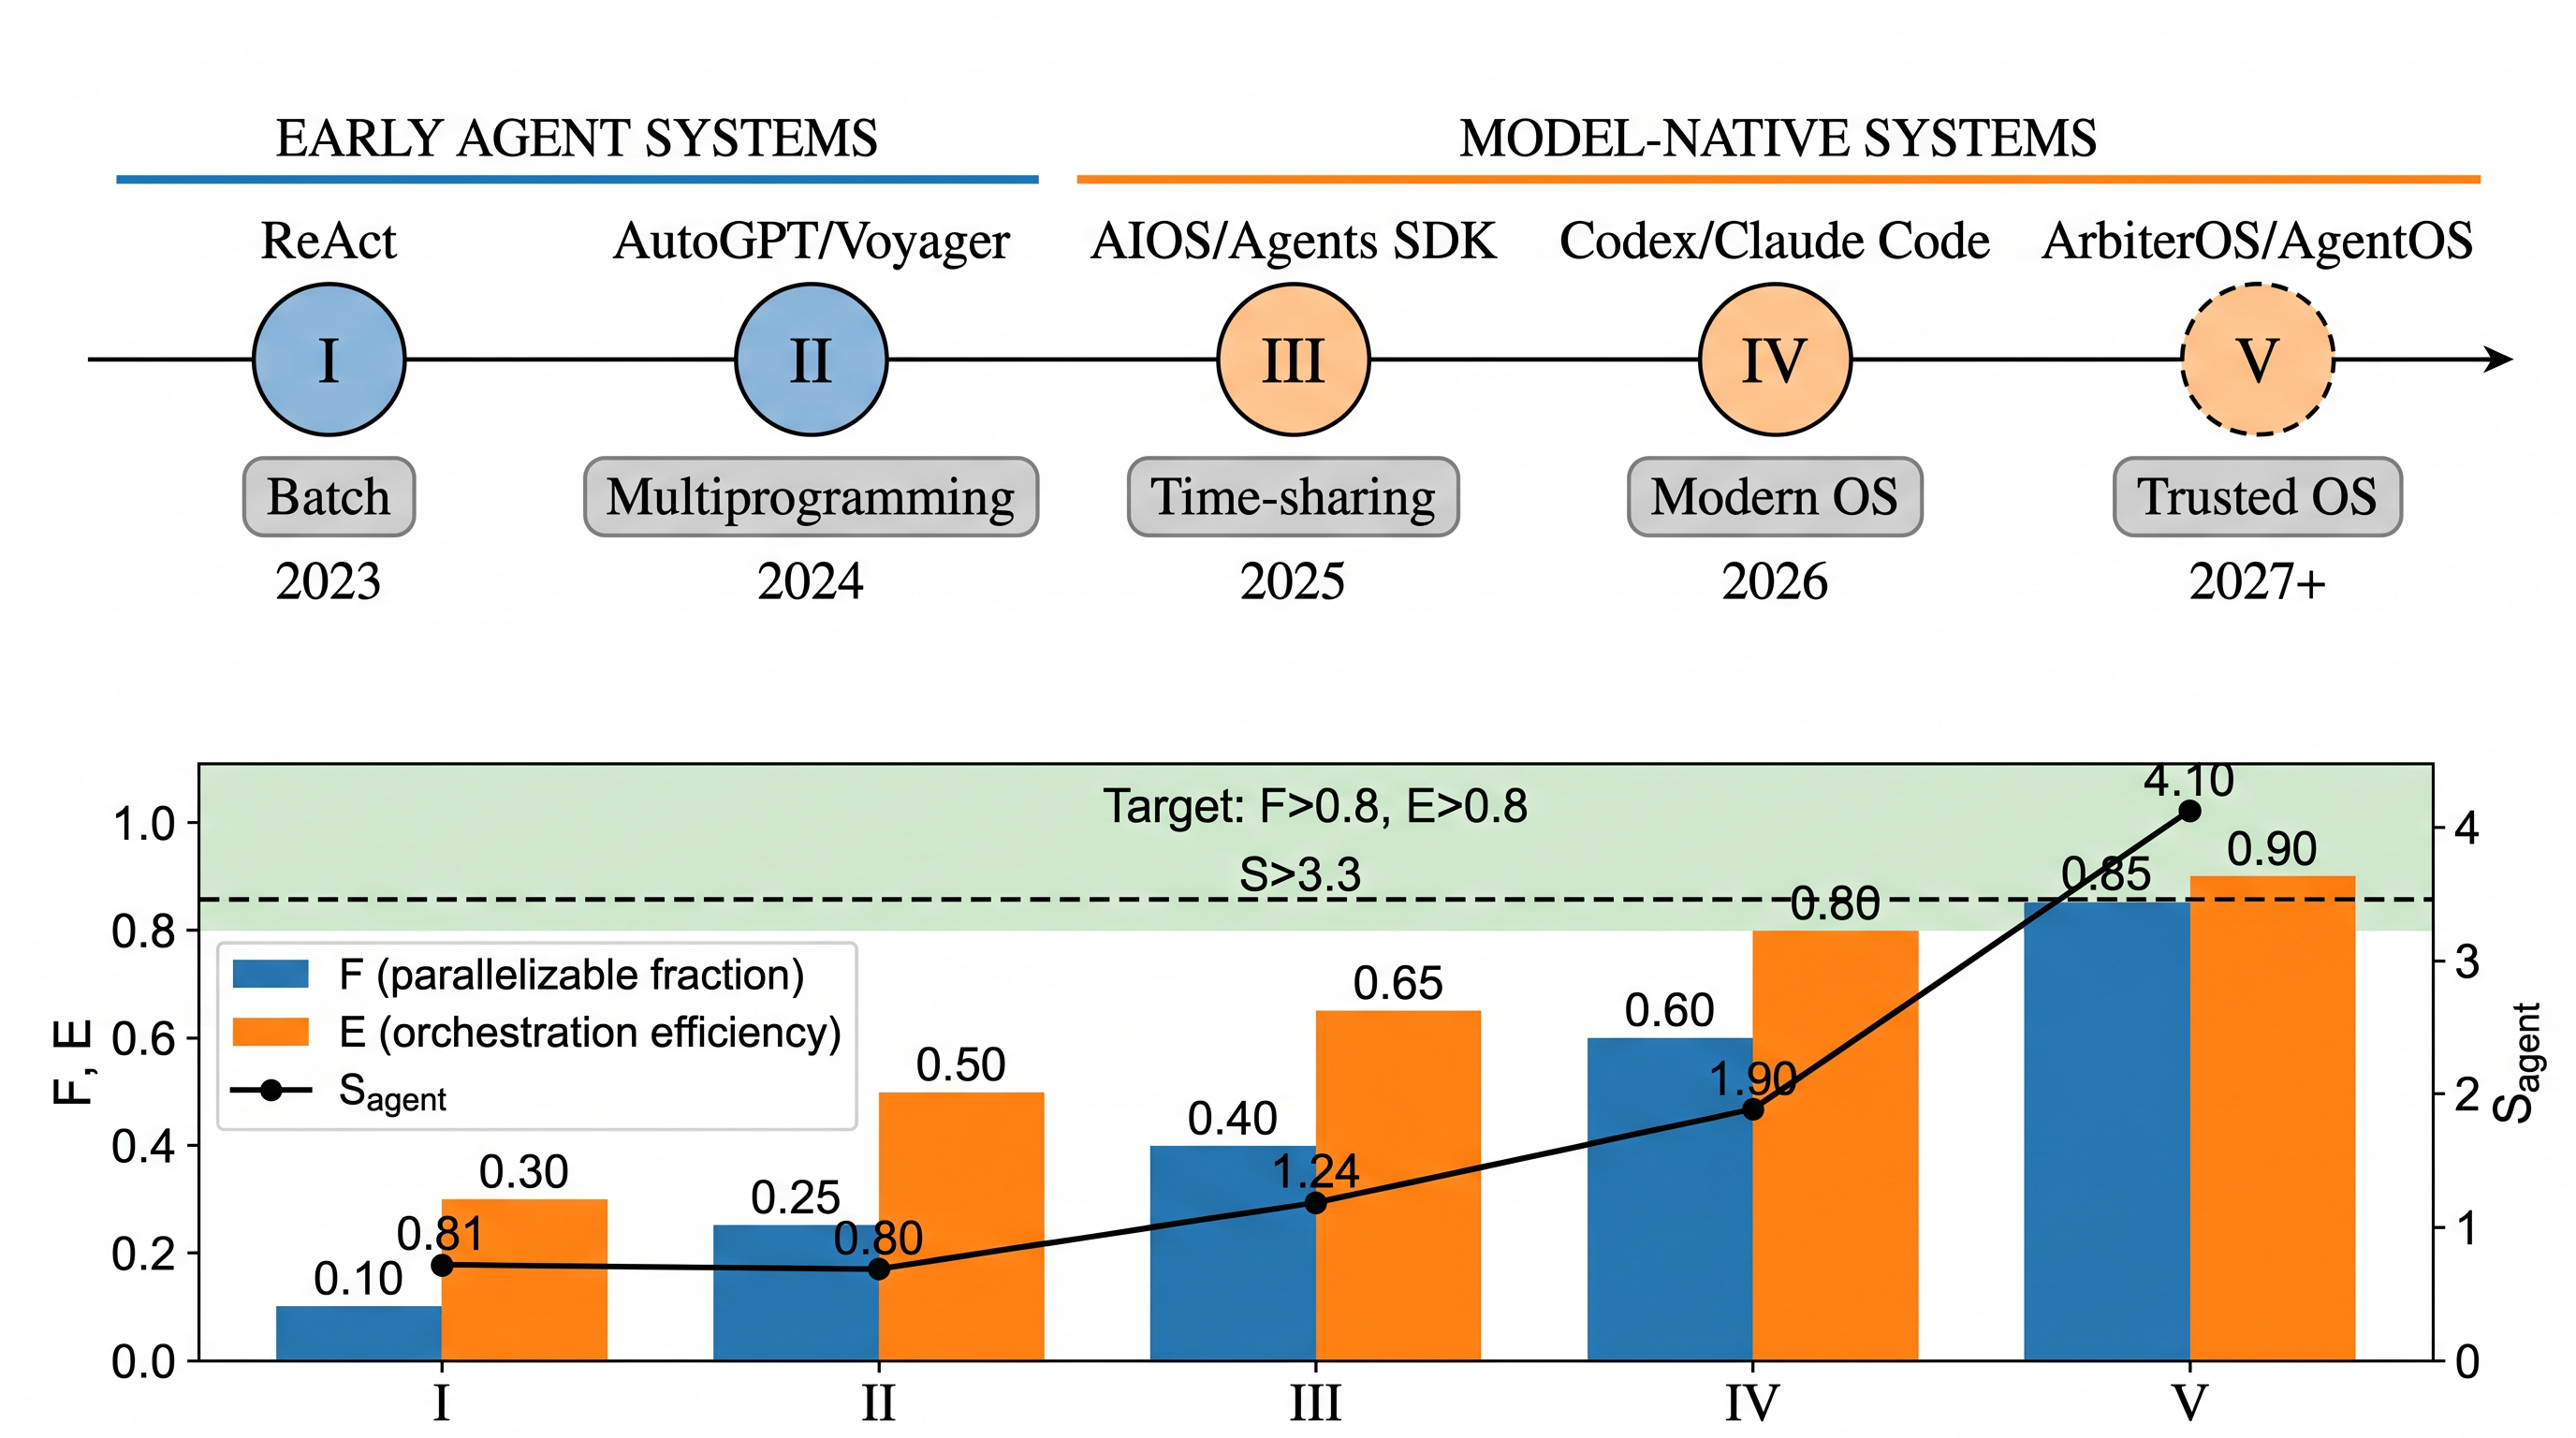
\includegraphics[width=0.95\textwidth]{figures/fig_agent_timeline_gemini.png}
%% ── Original TikZ version (commented out) ────────────────────────────────────
%\resizebox{0.95\textwidth}{!}{%
%\begin{tikzpicture}[
%    font=\sffamily,
%    >=Stealth,
%    milestone/.style={
%        circle,
%        minimum size=10mm,
%        inner sep=0pt,
%        line width=0.9pt,
%        font=\small\bfseries
%    },
%    early/.style={
%        milestone,
%        fill=softBlue,
%        draw=timelineBlue,
%        text=timelineBlue
%    },
%    native/.style={
%        milestone,
%        fill=softOrange,
%        draw=timelineOrange,
%        text=timelineOrange
%    },
%    future/.style={
%        native,
%        dashed
%    },
%    framework/.style={
%        align=center,
%        text width=29mm,
%        font=\small\bfseries,
%        text=timelineDark
%    },
%    oschip/.style={
%        rounded corners=2.5pt,
%        fill=softGray,
%        draw=timelineGray!65,
%        line width=0.45pt,
%        inner xsep=5pt,
%        inner ysep=2.6pt,
%        font=\scriptsize\itshape,
%        text=timelineDark,
%        align=center
%    },
%    year/.style={
%        font=\scriptsize\bfseries,
%        text=timelineGray!85!black
%    },
%    phase/.style={
%        font=\scriptsize\bfseries,
%        text=timelineDark
%    },
%    flow/.style={
%        -{Stealth[length=2.4mm,width=1.6mm]},
%        draw=timelineGray,
%        line width=0.95pt
%    }
%]

% Milestone nodes
%\node[early]  (g1) at (0.0,  0) {I};
%\node[early]  (g2) at (3.4,  0) {II};
%\node[native] (g3) at (6.8,  0) {III};
%\node[native] (g4) at (10.2, 0) {IV};
%\node[future] (g5) at (13.6, 0) {V};

% Evolution arrows
%\draw[flow] (g1.east) -- (g2.west);
%\draw[flow] (g2.east) -- (g3.west);
%\draw[flow] (g3.east) -- (g4.west);
%\draw[flow] (g4.east) -- (g5.west);

% Framework names
%\node[framework, above=5mm of g1] {ReAct};
%\node[framework, above=5mm of g2] {AutoGPT\\Voyager};
%\node[framework, above=5mm of g3] {AIOS\\Agents SDK};
%\node[framework, above=5mm of g4] {Codex\\Claude Code};
%\node[framework, above=5mm of g5] {ArbiterOS\\AgentOS};

% Operating-system analogies
%\node[oschip, below=8mm of g1] (o1) {Batch};
%\node[oschip, below=8mm of g2] (o2) {Multiprogramming};
%\node[oschip, below=8mm of g3] (o3) {Time-sharing};
%\node[oschip, below=8mm of g4] (o4) {Modern OS};
%\node[oschip, below=8mm of g5] (o5) {Trusted OS};

% Years
%\node[year, below=4mm of o1] {2023};
%\node[year, below=4mm of o2] {2024};
%\node[year, below=4mm of o3] {2025};
%\node[year, below=4mm of o4] {2026};
%\node[year, below=4mm of o5] {2027+};

% Phase headers
%\draw[timelineBlue, line width=0.95pt]
%    (-0.45, 2.28) -- (4.65, 2.28);
%\node[phase, text=timelineBlue]
%    at (2.10, 2.55) {EARLY AGENT SYSTEMS};

%\draw[timelineOrange, line width=0.95pt]
%    (5.95, 2.28) -- (14.05, 2.28);
%\node[phase, text=timelineOrange]
%    at (10.00, 2.55) {MODEL-NATIVE SYSTEMS};

%% ===========================================================
%% BOTTOM ROW: Quantitative F / E / S_agent chart (pgfplots)
%% ===========================================================
%% S_agent values computed via Law III:  S = 1/((1-F)+F/(N*E))
%%   Gen I:   N=1,  F=0.10, E=0.30 => S=0.81
%%   Gen II:  N=1,  F=0.25, E=0.50 => S=0.80
%%   Gen III: N=3,  F=0.40, E=0.65 => S=1.24
%%   Gen IV:  N=6,  F=0.60, E=0.80 => S=1.90
%%   Gen V:   N=10, F=0.85, E=0.90 => S=4.10

% ---- Left axis: F and E bars ----
%\begin{axis}[
%    name=barchart,
%    at={(-1.2,-8.0)},
%    anchor=north west,
%    width=15.6cm,
%    height=5.8cm,
%    ybar,
%    bar width=7pt,
%    ymin=0, ymax=1.08,
%    xmin=-0.5, xmax=4.5,
%    xtick={0,1,2,3,4},
%    xticklabels={I, II, III, IV, V},
%    xticklabel style={font=\sffamily\small\bfseries, color=timelineDark},
%    ytick={0,0.2,0.4,0.6,0.8,1.0},
%    yticklabels={0, 0.2, 0.4, 0.6, 0.8, 1.0},
%    yticklabel style={font=\sffamily\scriptsize, color=timelineDark},
%    ylabel={\small $F$,\; $E$},
%    ylabel style={font=\sffamily\small, color=timelineDark, at={(0.06,0.5)}},
%    axis y line*=left,
%    axis x line*=bottom,
%    enlarge x limits=0.15,
%    legend style={
%        at={(0.02,0.55)},
%        anchor=north west,
%        font=\sffamily\scriptsize,
%        draw=timelineGray!50,
%        fill=white,
%        fill opacity=0.9,
%        text opacity=1,
%        row sep=1pt,
%        /tikz/every even column/.append style={column sep=4pt}
%    },
%    tick style={draw=none},
%    major grid style={draw=timelineGray!20, line width=0.3pt},
%    ymajorgrids=true,
%    clip=false,
%]

% --- Target zone (F>0.8 and E>0.8 shaded region) ---
%\fill[green!12, opacity=0.5]
%    (axis cs:-0.5,0.8) rectangle (axis cs:4.5,1.08);
%\draw[green!50!black, densely dashed, line width=0.5pt]
%    (axis cs:-0.5,0.8) -- (axis cs:4.5,0.8);
% Label at top-right of green band, above the bars
%\node[font=\sffamily\tiny\itshape, text=green!40!black, anchor=north east]
%    at (axis cs:4.5,1.08) {Target: $F{>}0.8,\;E{>}0.8$};

% --- F bars (parallelizable fraction) ---
%\addplot[
%    fill=timelineBlue!55,
%    draw=timelineBlue,
%    line width=0.4pt
%] coordinates {
%    (0, 0.10)
%    (1, 0.25)
%    (2, 0.40)
%    (3, 0.60)
%    (4, 0.85)
%};
%\addlegendentry{$F$ (parallelizable fraction)}

% --- E bars (orchestration efficiency) ---
%\addplot[
%    fill=timelineOrange!55,
%    draw=timelineOrange,
%    line width=0.4pt
%] coordinates {
%    (0, 0.30)
%    (1, 0.50)
%    (2, 0.65)
%    (3, 0.80)
%    (4, 0.90)
%};
%\addlegendentry{$E$ (orchestration efficiency)}

%\end{axis}

% ---- Right axis: S_agent line ----
%\begin{axis}[
%    at={(barchart.south east)},
%    anchor=south east,
%    width=15.6cm,
%    height=5.8cm,
%    ymin=0, ymax=4.5,
%    xmin=-0.5, xmax=4.5,
%    xtick=\empty,
%    ytick={0,1,2,3,4},
%    yticklabels={$0$,$1$,$2$,$3$,$4$},
%    yticklabel style={font=\sffamily\scriptsize, color=timelineDark},
%    ylabel={\small $S_{\mathrm{agent}}$},
%    ylabel style={font=\sffamily\small, color=timelineDark, at={(0.96,0.5)}},
%    axis y line*=right,
%    axis x line=none,
%    enlarge x limits=0.15,
%    clip=false,
%    legend style={
%        at={(0.98,0.98)},
%        anchor=north east,
%        font=\sffamily\scriptsize,
%        draw=timelineGray!50,
%        fill=white,
%        fill opacity=0.9,
%        text opacity=1,
%        row sep=1pt
%    },
%]

% --- S_agent smooth line ---
%\addplot[
%    thick,
%    timelineDark,
%    mark=*,
%    mark size=2.5pt,
%    mark options={fill=timelineDark},
%    line width=1.1pt,
%    smooth
%] coordinates {
%    (0, 0.81)
%    (1, 0.80)
%    (2, 1.24)
%    (3, 1.90)
%    (4, 4.10)
%};
%\addlegendentry{$S_{\mathrm{agent}}$}

% --- S_agent value labels ---
%\node[font=\sffamily\tiny\bfseries, text=timelineDark, anchor=south]
%    at (axis cs:0,0.81) {0.81};
%\node[font=\sffamily\tiny\bfseries, text=timelineDark, anchor=south]
%    at (axis cs:1,0.80) {0.80};
%\node[font=\sffamily\tiny\bfseries, text=timelineDark, anchor=south]
%    at (axis cs:2,1.24) {1.24};
%\node[font=\sffamily\tiny\bfseries, text=timelineDark, anchor=south]
%    at (axis cs:3,1.90) {1.90};
%\node[font=\sffamily\tiny\bfseries, text=timelineDark, anchor=south]
%    at (axis cs:4,4.10) {4.10};

% --- Target S_agent dashed line at S=3.3 ---
%\draw[timelineDark, densely dotted, line width=0.6pt]
%    (axis cs:-0.5,3.3) -- (axis cs:4.5,3.3);
%\node[font=\sffamily\tiny\itshape, text=timelineDark, anchor=east]
%    at (axis cs:4.5,3.5) {$S{>}3.3$};

%\end{axis}

%\end{tikzpicture}}% end resizebox
\caption{Agent framework evolution from single-turn reasoning to model-native operating systems.
\textbf{Top:} representative frameworks with analogous OS milestones.
\textbf{Bottom:} quantitative trajectory of parallelizable fraction ($F$), orchestration efficiency ($E$), and agent speedup ($S_{\mathrm{agent}}$) per Law~III; green band marks the target regime ($F{>}0.8,\;E{>}0.8$).}
\label{fig_agent_timeline}
\end{figure}


%% ---------- Generation 1 ----------
\subsection{Generation I: Establishing the Execution Paradigm (2022--2023)}

\paragraph{Core contribution.}
The first generation of agent frameworks established the interleaved \textit{Thought--Action--Observation} loop as the fundamental execution paradigm.
Prior to this, LLM usage followed a single-turn, question-answer pattern: the user supplied a prompt, and the model returned a complete response, analogous to submitting a batch job and waiting for its output.
Generation~I broke this limitation by placing the model inside an active loop in which it could \textbf{reason} (analyze the current state and decide on the next step), \textbf{act} (invoke a tool or execute an operation), and \textbf{observe} (read the tool's return value), before entering the next iteration.

\paragraph{Representative systems.}
ReAct~\cite{yao2023react} is the foundational work of this generation.
Its core mechanism injects a ``Thought'' field into the prompt template, requiring the model to emit an explicit reasoning trace before every tool invocation.
When asked, for example, ``What is Shakespeare's longest play?'', the model does not guess the answer outright; instead, it first outputs ``I need to search for the lengths of all Shakespeare's plays,'' calls a search tool, and then reasons over the results to arrive at the final answer.
This ``think before you act'' discipline, while seemingly simple, effectively mitigates the \textit{hallucinated tool calls} that arise when models generate tool invocations without intermediate deliberation.
Toolformer~\cite{schick2023toolformer} approached the problem from a complementary angle: it taught the model \textbf{when and how} to invoke tools by injecting tool-call demonstrations into the training corpus, thereby acquiring tool usage as a self-supervised capability.

\paragraph{OS analogy.}
Generation~I frameworks correspond to the \textbf{single-task batch-processing systems} of the 1950s, such as the Fortran Monitor System on the IBM~704~\cite{ostep_2023}.
The system handles one task at a time, to completion, before starting the next; there is no concurrency, no interrupts, and no persistent state across tasks.
The ReAct loop is the simplest possible ``fetch--decode--execute'' pipeline, with each iteration analogous to a single instruction cycle.
There is no resource management whatsoever: no task scheduler (only one task exists), no memory management (the context window \textit{is} the entire ``memory''), and no I/O abstraction (tool calls are hard-coded).

%% ---------- Generation 2 ----------
\subsection{Generation II: Persistent Multi-Step Agents (2023)}

\paragraph{Core contribution.}
The defining advance of Generation~II is \textbf{persistence} and \textbf{autonomous goal decomposition}.
In Generation~I, each user query triggers an independent reasoning--action loop, and all intermediate state vanishes upon completion.
Generation~II frameworks allow agents to run continuously, autonomously decompose high-level goals into sequences of subtasks, maintain intermediate state across steps, and pass information between subtasks, in effect endowing the agent with a \textit{working memory}.

\paragraph{Representative systems.}
AutoGPT~\cite{autogpt_repo_2026} is the most widely recognized effort of this generation.
Given a high-level objective such as ``survey recent advances in quantum computing and write a report,'' AutoGPT autonomously decomposes it into subtasks (searching papers, extracting key findings, organizing an outline, and drafting the report) and executes them in sequence.
It introduces long-term memory backed by a vector database to store intermediate results across steps, enabling the agent to ``remember'' what it has already done.
However, AutoGPT also exposed Generation~II's central weakness: the absence of failure recovery.
Once a subtask goes wrong, the entire chain tends to spiral into infinite loops or accumulate compounding errors.

Voyager~\cite{wang2023voyager} made a critical improvement within the Minecraft environment by introducing a \textbf{skill library} (encapsulating successfully completed subtasks as reusable ``skills,'' analogous to function definitions) and an \textbf{automatic curriculum} that generates the next learning objective based on the agent's current capabilities, much like a pedagogical syllabus.
This enables the agent to accumulate experience incrementally rather than starting from scratch each time.
BabyAGI implemented a cleaner task-queue manager: maintaining a prioritized to-do list, executing tasks in priority order, and dynamically spawning new tasks based on execution results.

\paragraph{OS analogy.}
Generation~II corresponds to \textbf{multiprogramming} in the 1960s~\cite{ostep_2023}: the system begins to manage complex multi-step state, and tasks can share and pass information.
AutoGPT's task queue is a primitive ``job scheduler''; Voyager's skill library resembles an ``executable program library''; BabyAGI's priority ordering parallels early ``job scheduling policies.''
Compared with mature operating systems, however, Generation~II lacks three critical mechanisms: \textbf{isolation} (different tasks may interfere with one another), \textbf{preemptive scheduling} (a stalled task blocks the entire system), and \textbf{protection} (a failed task can corrupt the state of other tasks).

%% ---------- Generation 3 ----------
\subsection{Generation III: General-Purpose Runtimes (2023--2024)}

\paragraph{Core contribution.}
Generation~III frameworks systematically introduce \textbf{scheduling}, \textbf{isolation}, and \textbf{resource management}, upgrading the agent framework from a single-script automation tool into a general-purpose runtime platform.
The key indicator is that an agent is no longer merely a serial loop; it becomes a schedulable, suspendable, resumable ``process.''
Multiple agents can run concurrently without mutual interference, and the system explicitly manages computational resources such as inference budgets, context space, and tool-call rate limits.

\paragraph{Representative systems.}
AIOS~\cite{mei2024aios} constructed a complete agent operating system kernel organized into six subsystems: an Agent Scheduler for concurrent multi-agent scheduling, a Context Manager for context isolation and sharing across agents, a Memory Manager for hierarchical memory, a Tool Manager for tool registration and permission control, an I/O Manager for input--output mediation, and a Knowledge Manager for knowledge-base integration.
Each agent is encapsulated as a ``process'' with its own state space and resource budget.

The OpenAI Agents SDK~\cite{openai_codex_agentsdk_2026} pursued a more engineering-driven approach, packaging orchestration, state management, approval workflows, agent handoffs, and full-chain tracing into a code-first runtime.
Developers define agent behavioral specifications, permission boundaries, and collaboration protocols in Python, rather than encoding them implicitly through prompt templates.

AutoGen~\cite{wu2023autogen} proposed a multi-agent conversational framework in which multiple agents collaborate on complex tasks through structured message passing, each assuming a distinct role (e.g., programmer, tester, project manager), analogous to multi-process cooperation in a conventional operating system.

\paragraph{OS analogy.}
Generation~III corresponds to the \textbf{time-sharing operating systems} of the 1960s--70s, such as Multics and Unix~\cite{ostep_2023}.
The core breakthrough of time-sharing OSes was providing each user (process) with an independent address space and fair CPU time slices, enabling multiple users to safely share a single computer.
AIOS's Agent Scheduler corresponds to the process scheduler of a time-sharing OS; its Context Manager maps to the address isolation provided by the memory management unit (MMU); and the Tool Manager's permission controls parallel Unix's file permission system.
The Agents SDK's tracing mechanism mirrors OS-level system-call auditing via \texttt{strace} or \texttt{auditd}.

%% ---------- Generation 4 ----------
\subsection{Generation IV: Engineering-Grade Operating Systems (2024--2025)}

\paragraph{Core contribution.}
The hallmark of Generation~IV is \textbf{deep integration with real-world software engineering environments}.
Whereas the first three generations validated their concepts primarily in laboratory or constrained settings, Generation~IV confronts real codebases, real terminal environments, real file systems, and real external services.
This forces the system to address problems that earlier generations could sidestep: large repositories whose context far exceeds the model's window, tool calls that may produce irreversible side effects, concurrent edits that can introduce conflicts, and real projects that demand permission controls and audit trails.

\paragraph{Representative systems.}
OpenAI Codex~\cite{openai_codex_overview_2026} is a cloud-based coding agent that runs inside an isolated sandbox: it checks out the repository in a dedicated container, performs reads, writes, and command execution, and submits a diff for human review upon completion.
Codex introduced a sub-agent mechanism~\cite{openai_codex_overview_2026}: the primary agent can dispatch subtasks to specialized sub-agents, each running in its own sandbox, with results merged after approval, analogous to Unix's \texttt{fork()} creating child processes.
Codex also supports skills packages~\cite{openai_codex_skills_2026} and project-level instruction files (AGENTS.md)~\cite{openai_codex_agents_md_2026}, enabling reusable configurations across projects.

Claude Code~\cite{anthropic_claudecode_overview_2026} adopts a complementary design philosophy: it runs in the developer's local terminal, connects to external tools via the Model Context Protocol (MCP)~\cite{mcp_intro_2026}, defaults to read-only access (unless the user explicitly authorizes writes), and supports custom hooks that intercept and audit every tool call~\cite{anthropic_claudecode_security_2026}.
Claude Code's memory system~\cite{anthropic_claudecode_memory_2026} distinguishes between project-level memory (\texttt{CLAUDE.md}, analogous to a system configuration file) and user-level memory (cross-project personal preferences, analogous to dotfiles in the user's home directory).

OpenHands~\cite{openhands_paper_2025} provides an open agent platform supporting multiple model backends and sandbox environments; its OpenHands Index has become one of the standard benchmarks for evaluating coding agents.
OSWorld~\cite{osworld2024} advanced this direction from an evaluation standpoint by constructing real operating-system environments (complete with file managers, browsers, and terminals) and requiring agents to complete open-ended tasks within authentic GUI settings, thereby exposing agents' limitations when confronted with real-world complexity.
Devin~\cite{devin2024cognition} further exemplified Generation~IV's engineering orientation: as an ``AI software engineer,'' it integrates a code editor, browser, and terminal, and is capable of autonomous planning, coding, debugging, and deployment.

\paragraph{OS analogy.}
Generation~IV corresponds to the \textbf{modern operating systems} of the 1980s--90s, such as Unix System~V, early Linux, and Windows~NT~\cite{ostep_2023}.
The defining characteristic of modern OSes is their ability to handle real-world complexity: multitasking schedulers (e.g., the Completely Fair Scheduler~\cite{linux_cfs_2026}), virtual memory with demand paging, network protocol stacks, device driver frameworks, and security auditing.
Codex's sandbox maps to OS-level process isolation (each sub-agent runs in an independent container, akin to \texttt{chroot} or container technology); Claude Code's hooks parallel Linux Security Modules (LSM) security hooks; Codex's approval mechanism corresponds to Unix's \texttt{sudo} privilege escalation; and OpenHands's multi-model backend serves the role of a hardware abstraction layer (HAL).

%% ---------- Generation 5 ----------
\subsection{Generation V: Governed Operating Systems (2025--Present)}

\paragraph{Core contribution.}
The defining breakthrough of Generation~V is the elevation of security and governance from post-hoc patches to \textbf{first-principles architectural design}.
In the first four generations, security measures were additive: first make the agent functional, then bolt on sandboxes, approval gates, and audit logs.
Generation~V inverts this ordering: define security boundaries and governance rules first, then empower the agent to act within those boundaries.
This paradigm shift parallels the historical transition of operating systems from ``functional'' to ``trustworthy'': just as Multics introduced ring protection and mandatory access control in the 1960s, but it was not until the widespread adoption of SELinux and capability-based security that protection became an organic component of OS architecture~\cite{ostep_2023}.

\paragraph{Representative systems.}
ArbiterOS~\cite{arbiteros2025} explicitly articulates a layered architecture of ``probabilistic CPU + deterministic governor/kernel'': the underlying LLM serves as the probabilistic processor that determines \textit{what the agent can do}, while the governor above acts as the deterministic controller that decides \textit{what the agent should do}.
The governor constrains the agent's behavioral boundaries through policy specifications, analogous to how an OS kernel defines a process's capability envelope via system-call tables and permission bits.

AgentOS~\cite{agentos2025} introduces a reasoning kernel governed by structured operating-system logic, building system-level intelligent behavior upward from token-level context management.
Its central thesis is that an agent's reasoning process should not be an uncontrolled ``black-box loop,'' but rather managed through structured abstractions and interfaces, much like an OS kernel.

UFO$^2$~\cite{ufo2_2025}, targeting desktop environments, organizes the Desktop AgentOS into three tiers: a HostAgent as the top-level coordinator (analogous to the \texttt{init} process), AppAgents (one per application, analogous to service processes), and a GUI--API action layer at the bottom (analogous to the driver layer).
This stratification enables independent management and auditing of agent operations across different applications.

Aura~\cite{aura2025} realizes a security-first agent OS architecture on mobile devices, comprising a System Agent (with highest privilege), Sandboxed App Agents (one per application, akin to Android's application sandbox), and an Agent Kernel responsible for permission arbitration and resource allocation.
Aura emphasizes the unique risks of mobile environments: semantic input pollution (hijacking agent behavior through malicious inputs), memory taint propagation (compromised memory affecting all subsequent operations), and cross-application permission leakage.

CaMeL~\cite{debenedetti2025camel} derives its security model from first principles, proposing a capability-based model to defend against prompt-injection attacks.
Its core insight draws directly from capability-based security in operating systems: an agent cannot directly execute any operation with side effects, but must obtain a temporary capability token from a deterministic capability manager.
Each token authorizes only a single, specific operation (e.g., ``read-only access to file~X'') rather than granting blanket permissions.
This mirrors the evolution in Unix from the coarse-grained root/non-root privilege model to the fine-grained POSIX capabilities and SELinux mandatory access controls.

IronClaw~\cite{ironclaw2025} systematically argues why AI agents require operating-system-grade protection.
It observes that traditional software security assumes deterministic code with predictable behavior, whereas agent behavior is driven by probabilistic models.
The attack surface thus expands from ``code vulnerabilities'' to ``semantic vulnerabilities'': an adversary can hijack an agent's behavior through natural-language prompts without exploiting any code defect.

The OWASP \textbf{Agentic Applications Top~10}~\cite{owasp_agentic2026}, published in late 2025, further systematizes these threats into ten risk categories, including Agent Goal Hijack, Tool Misuse \& Exploitation, and Identity \& Privilege Abuse, providing a taxonomic foundation for the security design of Generation~V frameworks.

\paragraph{OS analogy.}
Generation~V corresponds to the inflection point at which operating systems transitioned from ``functional'' to ``trustworthy.''
In classical OS history, Unix~V6 (1975) was a functional but insecure system: it lacked memory protection (any process could read or write any memory address) and privilege separation (the root user held unrestricted power).
As networking and multi-user environments developed, security evolved from an ``optional feature'' to a ``foundational requirement,'' giving rise to Multics ring protection, SELinux mandatory access control, and formal verification of modern microkernels such as seL4~\cite{ostep_2023}.
Generation~V agent frameworks are undergoing the same transition: security is no longer merely ``add a sandbox,'' but requires a top-to-bottom redesign of the agent's permission model, audit mechanisms, and failure-recovery strategies at the architectural level.

%% ---------- Quantitative perspective ----------
Figure~\ref{fig_gen_matrix} summarises the capability maturity of each generation across six architectural dimensions.
\begin{figure}[htbp]
    \centering
    \resizebox{\textwidth}{!}{%
    \begin{tikzpicture}[
        cell/.style={
            minimum width=2.4cm, minimum height=1.0cm,
            align=center, font=\scriptsize,
            inner sep=2pt,
        },
        rowlabel/.style={
            % 【修复点】：将过宽的宽度大幅缩小至 2.8cm，彻底解决边框太宽和重叠问题
            minimum width=2.8cm, minimum height=1.0cm,
            text width=2.5cm, align=left, font=\small\bfseries,
            inner sep=4pt,
        },
        collabel/.style={
            minimum width=2.4cm, minimum height=0.9cm,
            align=center, font=\small\bfseries,
            inner sep=2pt,
        },
    ]
    
    % ── Capability columns ────────────────────────────────────────────────────────
    \def\cols{{"Task\\Decomp.", "Concurrency\\(F)", "Orchestration\\Eff.~(E)", "State\\Persist.", "Isolation\\/ Sandbox", "Security\\/ Govern."}}
    \def\ncols{6}
    
    % ── Color helper: 0=none, 1=low, 2=mid, 3=high ──────────────────────────────
    % 0 → white, 1 → 25%, 2 → 55%, 3 → 85% of modelnative
    \def\fillcol#1{%
        \ifnum#1=0 white\fi%
        \ifnum#1=1 modelnative!20\fi%
        \ifnum#1=2 modelnative!50\fi%
        \ifnum#1=3 modelnative!85\fi%
    }
    \def\txtcol#1{%
        \ifnum#1=0 gray!40\fi%
        \ifnum#1=1 modelnative!60!black\fi%
        \ifnum#1=2 modelnative!70!black\fi%
        \ifnum#1=3 white\fi%
    }
    \def\levelstr#1{%
        \ifnum#1=0 ---\fi%
        \ifnum#1=1 Low\fi%
        \ifnum#1=2 Medium\fi%
        \ifnum#1=3 High\fi%
    }
    
    % Data: rows = Gen I..V, each row = 6 values (0-3)
    % Gen I  (ReAct)
    \def\rowA{0,0,3,0,0,0}
    % Gen II (AutoGPT)
    \def\rowB{1,0,2,1,0,0}
    % Gen III (AIOS/SDK)
    \def\rowC{2,2,2,2,1,1}
    % Gen IV (Codex/Claude Code)
    \def\rowD{3,3,2,3,3,2}
    % Gen V (ArbiterOS/AURA)
    \def\rowE{3,3,3,3,3,3}
    
    \def\rowlabels{{"Gen~I\\(ReAct)", "Gen~II\\(AutoGPT)", "Gen~III\\(AIOS)", "Gen~IV\\(Codex)", "Gen~V\\(ArbiterOS)"}}
    \def\sublabels{{"2022--23", "2023", "2023--24", "2024--25", "2025--"}}
    
    % ── Draw column headers ───────────────────────────────────────────────────────
    \foreach \j/\lbl in {
        0/Task\\Decomp.,
        1/Concurrency\\$(F)$,
        2/Orchestration\\Eff.~$(E)$,
        3/State\\Persist.,
        4/Isolation\\/ Sandbox,
        5/Security\\/ Govern.}
    {
        \node[collabel, draw=gray!30, fill=gray!10]
            at ({3.9 + \j*2.4}, 0.5) {\lbl};
    }
    
    % Row label header
    % 【修复点】：X坐标整体向左平移至 1.3，与右侧列（起点 2.7）完美断开
    \node[rowlabel, draw=gray!30, fill=gray!10, minimum height=0.9cm]
        at (1.3, 0.5) {Generation};
    
    % ── Helper macro to draw one cell ────────────────────────────────────────────
    \newcommand{\drawcell}[3]{% #1=col(0-5), #2=row(0-4), #3=value(0-3)
        \pgfmathsetmacro\vint{int(#3)}%
        \ifnum\vint=0 \def\fc{white}\def\tc{gray!35}\fi%
        \ifnum\vint=1 \def\fc{modelnative!20}\def\tc{modelnative!65!black}\fi%
        \ifnum\vint=2 \def\fc{modelnative!50}\def\tc{modelnative!80!black}\fi%
        \ifnum\vint=3 \def\fc{modelnative!85}\def\tc{white}\fi%
        \node[cell, draw=gray!25, fill=\fc, text=\tc, minimum height=1.0cm]
            at ({3.9 + #1*2.4}, {-#2*1.0 - 0.5})
            {\ifnum\vint=0 ---\fi%
             \ifnum\vint=1 Low\fi%
             \ifnum\vint=2 Medium\fi%
             \ifnum\vint=3 High\fi};%
    }
    
    % ── Draw row labels ───────────────────────────────────────────────────────────
    \foreach \i/\rlab/\rsub in {
        0/{Gen~I}/{\footnotesize 2022--23},
        1/{Gen~II}/{\footnotesize 2023},
        2/{Gen~III}/{\footnotesize 2023--24},
        3/{Gen~IV}/{\footnotesize 2024--25},
        4/{Gen~V}/{\footnotesize 2025--Present}%
    }{
        \node[rowlabel, draw=gray!20, fill=gray!5, minimum height=1.0cm]
            at (1.3, {-\i*1.0 - 0.5})
            {\textbf{\rlab}\\[1pt]\rsub};
    }
    
    % ── Draw cells: \drawcell{col}{row}{value} ────────────────────────────────────
    % Gen I  (ReAct)
    \drawcell{0}{0}{0} \drawcell{1}{0}{0} \drawcell{2}{0}{3}
    \drawcell{3}{0}{0} \drawcell{4}{0}{0} \drawcell{5}{0}{0}
    
    % Gen II (AutoGPT/Voyager)
    \drawcell{0}{1}{1} \drawcell{1}{1}{0} \drawcell{2}{1}{2}
    \drawcell{3}{1}{1} \drawcell{4}{1}{0} \drawcell{5}{1}{0}
    
    % Gen III (AIOS/SDK)
    \drawcell{0}{2}{2} \drawcell{1}{2}{2} \drawcell{2}{2}{2}
    \drawcell{3}{2}{2} \drawcell{4}{2}{1} \drawcell{5}{2}{1}
    
    % Gen IV (Codex/Claude Code)
    \drawcell{0}{3}{3} \drawcell{1}{3}{3} \drawcell{2}{3}{2}
    \drawcell{3}{3}{3} \drawcell{4}{3}{3} \drawcell{5}{3}{2}
    
    % Gen V (ArbiterOS/AgentOS)
    \drawcell{0}{4}{3} \drawcell{1}{4}{3} \drawcell{2}{4}{3}
    \drawcell{3}{4}{3} \drawcell{4}{4}{3} \drawcell{5}{4}{3}
    
    % ── Legend (centred under table) ─────────────────────────────────────────────
    % 【修复点】：整体微调图例的坐标，使其严格居中对齐整个表格
    \node[font=\scriptsize, text=gray!60, anchor=east] at (5.7, -5.65) {Maturity:};
    \foreach \v/\lbl in {0/None, 1/Low, 2/Medium, 3/High} {
        \ifnum\v=0\def\fc{white}\def\tc{gray!40}\fi
        \ifnum\v=1\def\fc{modelnative!20}\def\tc{modelnative!65!black}\fi
        \ifnum\v=2\def\fc{modelnative!50}\def\tc{modelnative!80!black}\fi
        \ifnum\v=3\def\fc{modelnative!85}\def\tc{white}\fi
        \node[draw=gray!30, fill=\fc, text=\tc,
              minimum width=1.5cm, minimum height=0.55cm,
              font=\scriptsize, rounded corners=2pt]
            at ({6.7 + \v*1.9}, -5.65) {\lbl};
    }
    
    \end{tikzpicture}
    }% end resizebox
    \caption{Capability maturity matrix across the five generations of agent framework evolution. Each cell reflects the maturity level of a key architectural dimension: \textit{None} (---) through \textit{High}. The progressive darkening from Generation~I to Generation~V illustrates the systematic increase in both the parallelisable fraction~$F$ and the orchestration efficiency~$E$ captured by Law~III.}
    \label{fig_gen_matrix}
    \end{figure}

\subsection{The Five Generations Through the Lens of Law~III}

Viewed through the agent speedup law (Law~III) introduced in Section~\ref{sec:laws}, the five generations of evolution correspond to a progressive increase in $F$ (the parallelizable fraction) and $E$ (the orchestration efficiency).

Recall the formal statement of Law~III:
\begin{equation}
\label{eq:agent_law_review}
S_{\mathrm{agent}} = \frac{1}{(1-F) + \dfrac{F}{N \cdot E}}
\end{equation}
where $F \in [0,1]$ denotes the fraction of the task that can be decomposed for parallel execution, $N$ is the number of schedulable agents, and $E \in (0,1]$ is the orchestration efficiency ($E=1$ means zero overhead; $E\to 0$ means overhead consumes all parallel benefit).

\paragraph{Quantitative trajectory across generations.}
Figure~\ref{fig:gen_trajectory} plots the estimated values of $F$, $E$, and $S_{\mathrm{agent}}$ across the five generations.

% ---------------------------------------------------------------------------
% Five-Generation Quantitative Trajectory: F, E, S across Gen I–V
% fig:gen_trajectory
% ---------------------------------------------------------------------------
\begin{figure}[htbp]
\centering
\resizebox{0.88\textwidth}{!}{%
\begin{tikzpicture}
\small
\begin{groupplot}[
    group style={
        group size=3 by 1,
        horizontal sep=2.2cm,
    },
    width=5.0cm,
    height=5.2cm,
    grid=major,
    grid style={gray!18},
    tick label style={font=\footnotesize},
    label style={font=\small},
    xtick={1,2,3,4,5},
    xticklabels={I,II,III,IV,V},
    xlabel style={font=\small},
    ylabel style={font=\small},
    xmin=0.5, xmax=5.5,
    axis lines=left,
    every axis plot/.append style={thick, mark=*, mark size=2.2pt},
    enlargelimits=0.12,
    legend style={
        font=\scriptsize,
        at={(0.5,-0.32)},
        anchor=north,
        legend columns=1,
        draw=gray!40,
        rounded corners=2pt,
    },
]

%% (a) Parallelizable Fraction F
\nextgroupplot[
    title style={font=\small\bfseries, at={(0.5,1.06)}},
    title={(a) Parallelizable Fraction $F$},
    xlabel={Generation},
    ylabel={$F$},
    ymin=0, ymax=1.05,
    ytick={0,0.2,0.4,0.6,0.8,1.0},
]
\addplot[blue!70!black, mark=*]
    coordinates {(1,0.00)(2,0.15)(3,0.30)(4,0.50)(5,0.72)};
% target line
\addplot[red!60!black, dashed, no marks, domain=0.5:5.5] {0.8};
\addlegendentry{$F$ (estimated)}
\addlegendentry{Target $F>0.8$}
% annotations (shifted left)
\node[font=\tiny, blue!60!black, anchor=east] at (axis cs:0.9, 0.05) {${\approx}0$};
\node[font=\tiny, blue!60!black, anchor=east] at (axis cs:1.85, 0.20) {$0.15$};
\node[font=\tiny, blue!60!black, anchor=east] at (axis cs:2.85, 0.35) {$0.30$};
\node[font=\tiny, blue!60!black, anchor=east] at (axis cs:3.85, 0.53) {$0.50$};
\node[font=\tiny, blue!60!black, anchor=east] at (axis cs:4.85, 0.73) {$0.72$};

%% (b) Orchestration Efficiency E
\nextgroupplot[
    title style={font=\small\bfseries, at={(0.5,1.06)}},
    title={(b) Orchestration Efficiency $E$},
    xlabel={Generation},
    ylabel={$E$},
    ymin=0, ymax=1.05,
    ytick={0,0.2,0.4,0.6,0.8,1.0},
]
\addplot[orange!80!black, mark=square*]
    coordinates {(1,1.00)(2,0.90)(3,0.70)(4,0.50)(5,0.65)};
\addplot[red!60!black, dashed, no marks, domain=0.5:5.5] {0.8};
\addlegendentry{$E$ (estimated)}
\addlegendentry{Target $E>0.8$}
\node[font=\tiny, orange!70!black] at (axis cs:1, 0.88) {$1.0$};
\node[font=\tiny, orange!70!black] at (axis cs:2, 1) {$0.9$};
\node[font=\tiny, orange!70!black] at (axis cs:3, 0.58) {$0.7$};
\node[font=\tiny, orange!70!black] at (axis cs:4, 0.38) {$0.5$};
\node[font=\tiny, orange!70!black] at (axis cs:5, 0.5) {$0.65$};

%% (c) Agent Speedup S
\nextgroupplot[
    title style={font=\small\bfseries, at={(0.5,1.06)}},
    title={(c) Agent Speedup $S_{\mathrm{agent}}$},
    xlabel={Generation},
    ylabel={$S_{\mathrm{agent}}$},
    ymin=0, ymax=4.0,
    ytick={0,1,2,3,4},
]
\addplot[red!70!black, mark=triangle*, mark size=2.5pt]
    coordinates {(1,1.00)(2,1.00)(3,1.27)(4,1.60)(5,2.10)};
\addplot[red!50!black, dashed, no marks, domain=0.5:5.5] {3.3};
\addlegendentry{$S_{\mathrm{agent}}$}
\addlegendentry{Target $S>3.3$}
\node[font=\tiny, red!65!black] at (axis cs:1, 1.3) {$1.0$};
\node[font=\tiny, red!65!black] at (axis cs:2, 1.3) {$1.0$};
\node[font=\tiny, red!65!black] at (axis cs:3, 1.7) {$1.27$};
\node[font=\tiny, red!65!black] at (axis cs:4, 2.0) {$1.60$};
\node[font=\tiny, red!65!black] at (axis cs:5, 2.5) {$2.10$};

\end{groupplot}
\end{tikzpicture}}%
\caption{Quantitative trajectory of agent framework parameters across five generations, estimated from Law~III ($S_{\mathrm{agent}} = 1/((1-F)+F/(N{\cdot}E))$ with representative $N$ values per generation). (a)~Parallelizable fraction $F$ grows from near zero (Gen~I serial loop) to ${\approx}0.72$ (Gen~V governed OS). (b)~Orchestration efficiency $E$ initially near~1 (trivial single-agent overhead) but dips in Gen~IV due to sandbox isolation and approval overhead, then recovers in Gen~V with governance-first design. (c)~Resulting speedup $S_{\mathrm{agent}}$ rises from $1.0\times$ to ${\approx}2.1\times$, still well below the target $3.3\times$ that requires $F>0.8$ and $E>0.8$ simultaneously. Dashed red lines mark the target thresholds.}
\label{fig:gen_trajectory}
\end{figure}


\textit{Generation~I (ReAct).}
$F \approx 0$ (no task decomposition; single-agent serial execution), $N=1$, $E \approx 1$ (no orchestration overhead), yielding $S_{\mathrm{agent}} \approx 1$.
This corresponds to the ``uniprocessor, no parallelism'' regime.

\textit{Generation~II (AutoGPT/Voyager).}
$F \approx 0.1$--$0.2$ (a small fraction of subtasks can be separated), $N=1$ (still a single agent), $E \approx 0.9$, yielding $S_{\mathrm{agent}} \approx 1$.
Decomposition capability begins to emerge, but with only one agent there is no opportunity for parallel speedup.

\textit{Generation~III (AIOS/Agents SDK).}
$F \approx 0.3$ (moderate decomposition capability), $N \approx 2$--$4$ (multi-agent support emerges), $E \approx 0.7$ (scheduling and context switching introduce significant overhead), yielding $S_{\mathrm{agent}} \approx 1/(0.7 + 0.3/2.8) \approx 1.27$.
Multi-agent execution begins to deliver speedup, but orchestration overhead partially cancels the gains.

\textit{Generation~IV (Codex/Claude Code).}
$F \approx 0.5$ (real-world software engineering tasks exhibit substantial decomposability), $N \approx 4$--$8$ (sub-agent concurrency), $E \approx 0.5$ (sandbox isolation, approval workflows, and state synchronization impose significant overhead), yielding $S_{\mathrm{agent}} \approx 1/(0.5 + 0.5/4) \approx 1.6$.
Speedup becomes substantial, yet orchestration overhead remains the binding constraint.

\textit{Generation~V (ArbiterOS/CaMeL/IronClaw).}
$F \approx 0.72$ (governance-first design enables broader task decomposition), $N \approx 6$ (mature multi-agent concurrency), $E \approx 0.65$ (governance overhead partially recovered through structured policy enforcement and capability tokens), yielding $S_{\mathrm{agent}} \approx 1/(0.28 + 0.72/3.9) \approx 2.1$.
The partial recovery of $E$ relative to Gen~IV reflects the shift from ad-hoc sandboxing to principled capability-based security, which reduces redundant permission checks. However, $F$ and $E$ remain below the $0.8$ threshold required for the target $3.3\times$ speedup.

The execution time horizon of Generation~IV systems is also expanding from minutes to hours.
In a striking demonstration, engineers at Rakuten tested Claude Code on the vLLM project (12.5~million lines of code), where it ran autonomously for seven hours to complete an activation-vector extraction task, achieving 99.9\% numerical accuracy~\cite{anthropic2026agenticreport}.
This kind of long-duration autonomous execution introduces new architectural challenges, including cross-hour KV-cache persistence, checkpoint/recovery protocols, and sustained resource management, that further reinforce the analogy between agent runtimes and operating systems.

\paragraph{The target: a true model-native OS.}
Achieving a genuine model-native operating system requires $F > 0.8$ and $E > 0.8$, which would yield $S_{\mathrm{agent}} > 1/(0.2 + 0.8/8) \approx 3.3$.
This target demands both high decomposability (high~$F$) \textit{and} low orchestration overhead (high~$E$), a dual requirement that no current system meets.

Recent benchmark results on GAIA~\cite{gaia2023}, $\tau$-bench~\cite{taubench2024}, and SWE-bench~\cite{swebench2023} remind us how far current systems remain from this goal.
On SWE-bench Verified, the best-performing agent systems as of late 2025 achieve a pass rate of approximately 70--75\%, meaning that in roughly one quarter of real software engineering tasks, agents still cannot correctly decompose and execute the required work.
On $\tau$-bench, agent performance during multi-turn interactions with real users is even less stable, because the ambiguity of user instructions and the dynamism of the environment further depress both $F$ and $E$.
